\documentclass[11pt]{article}

\usepackage[margin=1in]{geometry}
\usepackage{amsmath, amssymb, amsthm}
\usepackage{graphicx}
\usepackage{booktabs}
\usepackage{caption}
\usepackage{subcaption}
\usepackage[hidelinks]{hyperref}
\usepackage{authblk}
\usepackage{float}
\usepackage[authoryear,round]{natbib}

\graphicspath{{../results/}}

\newtheorem{proposition}{Proposition}

\title{\textbf{Beyond Black--Scholes: A Computational Study of\\
Option Pricing under Stochastic Volatility and Jumps}}

\author{Chia-Jui Yeh}
\affil{\small Companion paper to the \texttt{options-pricing-engine} repository}
\date{June 2026}

\begin{document}
\maketitle

\begin{abstract}
\noindent
The Black--Scholes--Merton model remains the cornerstone of option pricing, yet
its assumption of constant volatility is flatly contradicted by the
\emph{volatility smile} observed in traded option markets. This paper documents a
self-contained pricing library that implements and cross-validates a hierarchy of
models and numerical methods: the Black--Scholes benchmark with analytic Greeks;
lattice, Monte Carlo, and quasi-Monte Carlo numerical schemes; the Heston
stochastic-volatility model priced by a semi-analytic Fourier integral; the
Merton jump-diffusion model; path-dependent (Asian, barrier, lookback) options;
and American options via Least-Squares Monte Carlo. Every method is validated
against an independent benchmark---Fourier prices against Monte Carlo, lattice
prices against closed forms, and simulation estimators against analytic control
variates. We apply the library to real S\&P~500 (SPY) option quotes and show that
the observed implied-volatility skew, which Black--Scholes cannot represent, is
reproduced by calibrating the Heston and Merton models to the market: a
vega-weighted least-squares fit attains $0.60\%$ and $1.22\%$ implied-volatility
RMSE respectively across 903 liquid quotes spanning six maturities. We further
demonstrate that a geometric-average control variate reduces Asian-option
simulation variance by a factor of roughly $36\times$, and that a scrambled Sobol
sequence improves the European-option convergence rate from $O(n^{-1/2})$ toward
$O(n^{-1})$. All inputs are real market data and all results are reproducible from
the accompanying open-source code.
\end{abstract}

\section{Introduction}

The 1973 Black--Scholes--Merton (BSM) framework \citep{blackscholes1973,
merton1973} gives a closed-form price for European options under the assumption
that the underlying asset follows a geometric Brownian motion with constant
volatility. Its elegance and tractability made it the lingua franca of
derivatives markets. However, two robust empirical facts contradict its
assumptions. First, implied volatilities backed out of market prices are not
constant across strikes: out-of-the-money equity puts trade at systematically
higher implied volatilities than at-the-money options, producing the
characteristic \emph{volatility skew}. Second, asset returns exhibit heavy tails
and sudden discontinuities that a pure diffusion cannot generate.

Two families of models address these deficiencies. \emph{Stochastic-volatility}
models, of which the Heston \citep{heston1993} model is the canonical example,
let the instantaneous variance follow its own mean-reverting diffusion correlated
with the asset. \emph{Jump-diffusion} models, introduced by
\citet{merton1976}, superimpose a compound Poisson process of discontinuous jumps
on the diffusion. Both generate non-constant implied-volatility curves and richer
return distributions.

This paper accompanies an open-source pricing library and serves two purposes.
Pedagogically, it derives and connects the main pricing techniques used on a
modern derivatives desk. Empirically, it demonstrates---with reproducible
numerical experiments---how the advanced models cure the shortcomings of
Black--Scholes, and how careful numerical design (variance reduction,
low-discrepancy sequences, regression-based early-exercise rules) makes these
models computationally practical. The guiding methodological principle is
\emph{cross-validation}: wherever a quantity can be computed two independent
ways, we compute it both ways and verify agreement.

The remainder of the paper is organised as follows.
Section~\ref{sec:bs} reviews the Black--Scholes benchmark and its Greeks.
Section~\ref{sec:numerics} covers the lattice, Monte Carlo, and quasi-Monte Carlo
methods used throughout. Section~\ref{sec:beyond} introduces the Heston and
Merton models and shows that they reproduce the smile. Section~\ref{sec:exotic}
treats path-dependent and American options. Section~\ref{sec:empirical} calibrates
the Heston and Merton models to real S\&P~500 option data. Section~\ref{sec:results}
collects the numerical results and Section~\ref{sec:conclusion} concludes.

\section{The Black--Scholes Benchmark}
\label{sec:bs}

Under the risk-neutral measure $\mathbb{Q}$, the underlying follows
\begin{equation}
\mathrm{d}S_t = (r-q) S_t\,\mathrm{d}t + \sigma S_t\,\mathrm{d}W_t,
\end{equation}
where $r$ is the risk-free rate, $q$ the continuous dividend yield, and $\sigma$
the (constant) volatility. The time-$0$ price of a European call with strike $K$
and maturity $T$ is
\begin{equation}
C = S_0 e^{-qT}\Phi(d_1) - K e^{-rT}\Phi(d_2), \qquad
d_{1,2} = \frac{\ln(S_0/K) + (r-q\pm\tfrac12\sigma^2)T}{\sigma\sqrt{T}},
\label{eq:bs}
\end{equation}
with $\Phi$ the standard normal CDF and the put price following from put--call
parity, $C - P = S_0 e^{-qT} - K e^{-rT}$.

\paragraph{Greeks.} The library computes the analytic sensitivities
$\Delta=\partial C/\partial S$, $\Gamma=\partial^2 C/\partial S^2$,
$\mathcal{V}=\partial C/\partial \sigma$ (vega), $\Theta=\partial C/\partial t$,
and $\rho=\partial C/\partial r$ in closed form. These serve both for hedging and
as a consistency check: e.g.\ $\Gamma$ is identical for calls and puts, and
$0<\Delta_{\text{call}}<1$ while $-1<\Delta_{\text{put}}<0$, both verified in the
test suite. Figure~\ref{fig:greeks} plots the principal Greeks against spot: the
call delta rises sigmoidally from $0$ to $1$ as the option moves into the money,
while gamma and vega---the second-order and volatility sensitivities---peak near
the money, where optionality is greatest, and decay in both tails.

\begin{figure}[H]
\centering
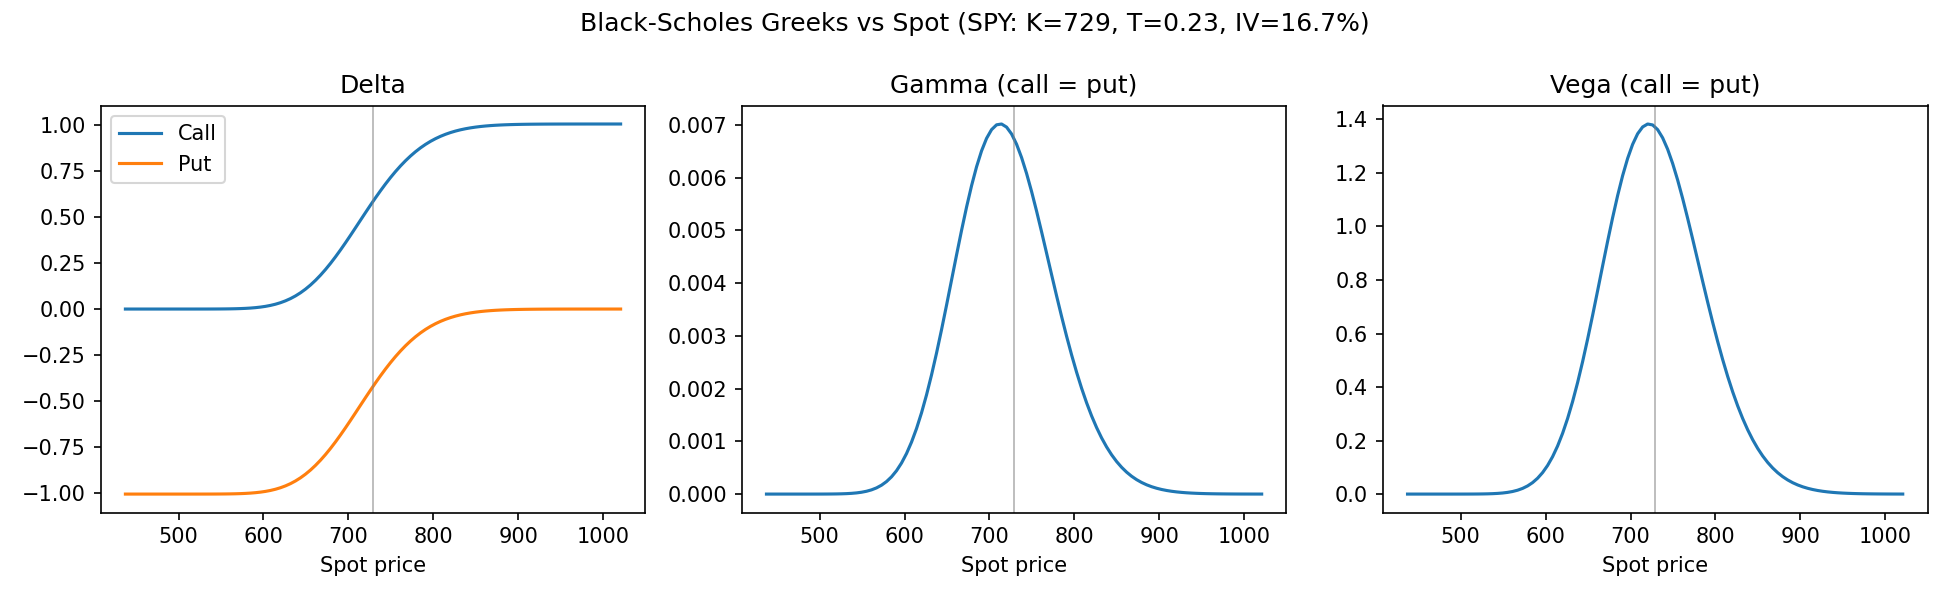
\includegraphics[width=\textwidth]{greeks_profiles.png}
\caption{Black--Scholes Greeks as a function of spot ($K=100$, $T=1$,
$\sigma=20\%$). Delta is bounded in $(0,1)$ for the call and $(-1,0)$ for the
put; gamma and vega are identical for calls and puts and are maximal near the
money.}
\label{fig:greeks}
\end{figure}

\paragraph{Implied volatility.} Given a market price, the implied volatility is
the $\sigma$ solving \eqref{eq:bs}. We invert it by Newton--Raphson using the
analytic vega, falling back to Brent's method on the rare occasions vega is too
small for stable Newton steps (deep out-of-the-money, short maturity). The
implied-volatility map is the lens through which all later models are compared:
each model's prices are converted to BSM-implied volatilities and plotted against
strike.

\section{Numerical Methods}
\label{sec:numerics}

\subsection{Binomial lattice}
The Cox--Ross--Rubinstein (CRR) tree \citep{crr1979} discretises
$[0,T]$ into $N$ steps with up/down factors $u=e^{\sigma\sqrt{\Delta t}}$,
$d=1/u$ and risk-neutral probability
$p=(e^{(r-q)\Delta t}-d)/(u-d)$. The option value is computed by backward
induction. The lattice converges to \eqref{eq:bs} as $N\to\infty$ at rate
$O(1/N)$ (with the familiar even/odd oscillation), confirmed in
Figure~\ref{fig:binomial}. Its practical importance is that it handles
\emph{American} exercise directly by taking the maximum of continuation and
intrinsic value at every node---something the closed form cannot do.

\subsection{Monte Carlo and variance reduction}
Monte Carlo estimates the discounted risk-neutral expectation
$e^{-rT}\mathbb{E}^{\mathbb{Q}}[\,\text{payoff}\,]$ by simulation. Its error
decays as $O(n^{-1/2})$ in the number of paths $n$, so variance reduction is
essential. We implement two standard techniques:
\begin{itemize}
\item \textbf{Antithetic variates}: pairing each normal draw $Z$ with $-Z$ removes
sampling asymmetry and halves the effective variance for monotone payoffs.
\item \textbf{Control variates}: subtracting a correlated quantity with known
expectation. For a European call the discounted terminal spot is an exact control
($\mathbb{E}[e^{-rT}S_T]=S_0 e^{-qT}$); for an arithmetic Asian option the
\emph{geometric} Asian option---which has a closed form---is a near-perfect
control (Section~\ref{sec:exotic}).
\end{itemize}

\subsection{Quasi-Monte Carlo}
Replacing pseudo-random draws with a low-discrepancy \emph{Sobol} sequence (with
Owen scrambling, inverted through $\Phi^{-1}$) accelerates convergence for
smooth, low-dimensional integrands. For the one-dimensional European payoff we
observe (Figure~\ref{fig:qmc}) the error decaying close to $O(n^{-1})$ rather
than $O(n^{-1/2})$---two orders of magnitude fewer samples for the same accuracy
at $n\sim10^4$.

\section{Beyond Black--Scholes}
\label{sec:beyond}

\subsection{The Heston stochastic-volatility model}
Heston \citep{heston1993} models the variance $v_t$ as a Cox--Ingersoll--Ross
diffusion correlated with the asset:
\begin{align}
\mathrm{d}S_t &= (r-q) S_t\,\mathrm{d}t + \sqrt{v_t}\,S_t\,\mathrm{d}W_t^S,\\
\mathrm{d}v_t &= \kappa(\theta - v_t)\,\mathrm{d}t + \xi\sqrt{v_t}\,\mathrm{d}W_t^v,
\qquad \mathrm{d}\langle W^S, W^v\rangle_t = \rho\,\mathrm{d}t,
\end{align}
with mean-reversion speed $\kappa$, long-run variance $\theta$, vol-of-vol $\xi$,
and leverage correlation $\rho$ (typically negative for equities). The parameter
$\rho$ controls the skew and $\xi$ the convexity of the smile; the Feller
condition $2\kappa\theta>\xi^2$ guarantees $v_t>0$.

Heston's tractability comes from the closed-form characteristic function of the
log-price $x_T=\ln S_T$. Writing $\phi(u)=\mathbb{E}[e^{iu x_T}]$, the price
admits the Fourier representation
\begin{equation}
C = S_0 e^{-qT} P_1 - K e^{-rT} P_2, \qquad
P_j = \frac12 + \frac{1}{\pi}\int_0^\infty
\operatorname{Re}\!\left[\frac{e^{-iu\ln K}\,\phi_j(u)}{iu}\right]\mathrm{d}u,
\label{eq:heston}
\end{equation}
where $\phi_2=\phi$ and $\phi_1(u)=\phi(u-i)/\phi(-i)$, and $\phi(-i)=S_0
e^{(r-q)T}$. We evaluate \eqref{eq:heston} with adaptive quadrature, using the
Albrecher et al.\ \citep{albrecher2007} ``good'' formulation of $\phi$ that
avoids the branch-cut discontinuity (the ``Little Heston Trap'') and is stable at
long maturities. As an independent check, a full-truncation Euler Monte Carlo
\citep{lord2010} reprices the same options; the two agree to within Monte Carlo
error plus a small discretisation bias (Section~\ref{sec:results}).

\subsection{The Merton jump-diffusion model}
Merton \citep{merton1976} adds log-normal jumps arriving as a Poisson process of
intensity $\lambda$:
\begin{equation}
\frac{\mathrm{d}S_t}{S_{t^-}} = (r-q-\lambda k)\,\mathrm{d}t + \sigma\,\mathrm{d}W_t
+ (J-1)\,\mathrm{d}N_t, \qquad \ln J \sim \mathcal{N}(\mu_J,\sigma_J^2),
\end{equation}
with compensator $k=\mathbb{E}[J-1]=e^{\mu_J+\sigma_J^2/2}-1$ ensuring the
discounted price is a martingale. Conditioning on the number of jumps yields
Merton's series, a Poisson-weighted sum of Black--Scholes prices,
\begin{equation}
C = \sum_{n=0}^{\infty}\frac{e^{-\lambda' T}(\lambda' T)^n}{n!}\,
C_{\text{BS}}\!\left(S_0,K,T,r_n,\sigma_n\right),
\label{eq:merton}
\end{equation}
where $\lambda'=\lambda(1+k)$,
$\sigma_n^2=\sigma^2+n\sigma_J^2/T$, and $r_n=r-\lambda k+n(\mu_J+\tfrac12\sigma_J^2)/T$.
The use of the jump-adjusted intensity $\lambda'$ (rather than $\lambda$) in the
Poisson weights is precisely what makes the per-term discounting consistent; an
independent terminal-value Monte Carlo confirms the series
(Section~\ref{sec:results}).

\subsection{Reproducing the volatility smile}
Both models break the constant-volatility straitjacket: pricing options across
strikes and inverting to BSM-implied volatility yields a non-flat curve. The
calibrated-Heston implied-volatility surface (Figure~\ref{fig:surface}) shows a
pronounced downward skew, steepest at short maturities and flattening as $T$
grows, matching the documented term structure of equity-index skew.
Section~\ref{sec:empirical} confirms this directly against real S\&P~500 quotes
and reports the calibration quality.

The mechanism behind the smile is visible in the risk-neutral return
distribution. Figure~\ref{fig:returns} compares the simulated terminal
log-returns under the three models, all parameterised by the SPY calibration of
Section~\ref{sec:empirical}. Black--Scholes is Gaussian by construction; Heston,
through its negative leverage correlation, is left-skewed, placing more mass on
large downward moves and thereby richening out-of-the-money puts; Merton's jumps
produce a sharply peaked body with heavy tails. It is precisely these departures
from normality---skewness and excess kurtosis---that translate, through the
inversion of \eqref{eq:bs}, into the observed implied-volatility skew.

\begin{figure}[H]
\centering
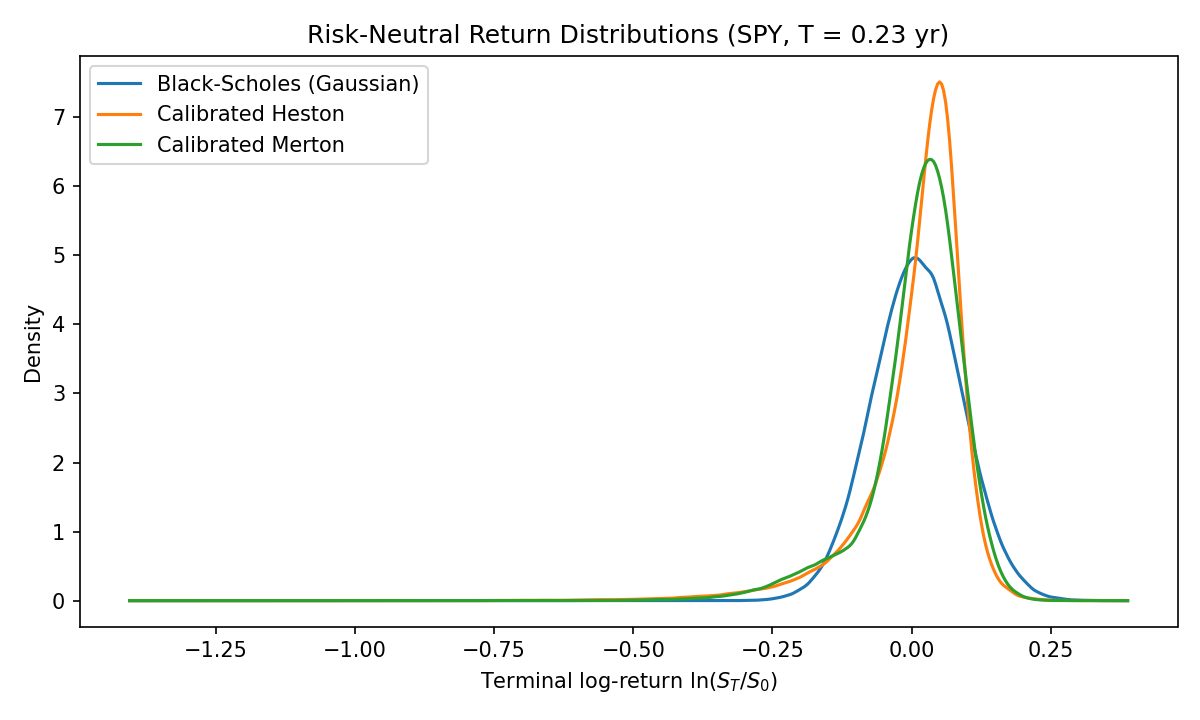
\includegraphics[width=0.78\textwidth]{return_distributions.png}
\caption{Risk-neutral densities of the terminal log-return $\ln(S_T/S_0)$ at the
SPY reference maturity ($T=0.23$), using the calibrated parameters. Heston is
left-skewed and Merton fat-tailed relative to the Gaussian Black--Scholes
benchmark; these shape deviations are the source of the skew.}
\label{fig:returns}
\end{figure}

The two Heston parameters that shape the smile play distinct, interpretable
roles, illustrated in Figure~\ref{fig:sensitivity}. The leverage correlation
$\rho$ tilts the smile: $\rho<0$ produces the downward equity skew, $\rho>0$ an
upward skew, and $\rho=0$ a symmetric smile. The vol-of-vol $\xi$ governs
convexity: raising $\xi$ fattens both tails and deepens the curvature of the
smile, while leaving the at-the-money level largely unchanged. This decoupling is
what makes the model practically calibratable---$\rho$ and $\xi$ target the slope
and curvature of the observed surface almost independently.

\begin{figure}[H]
\centering
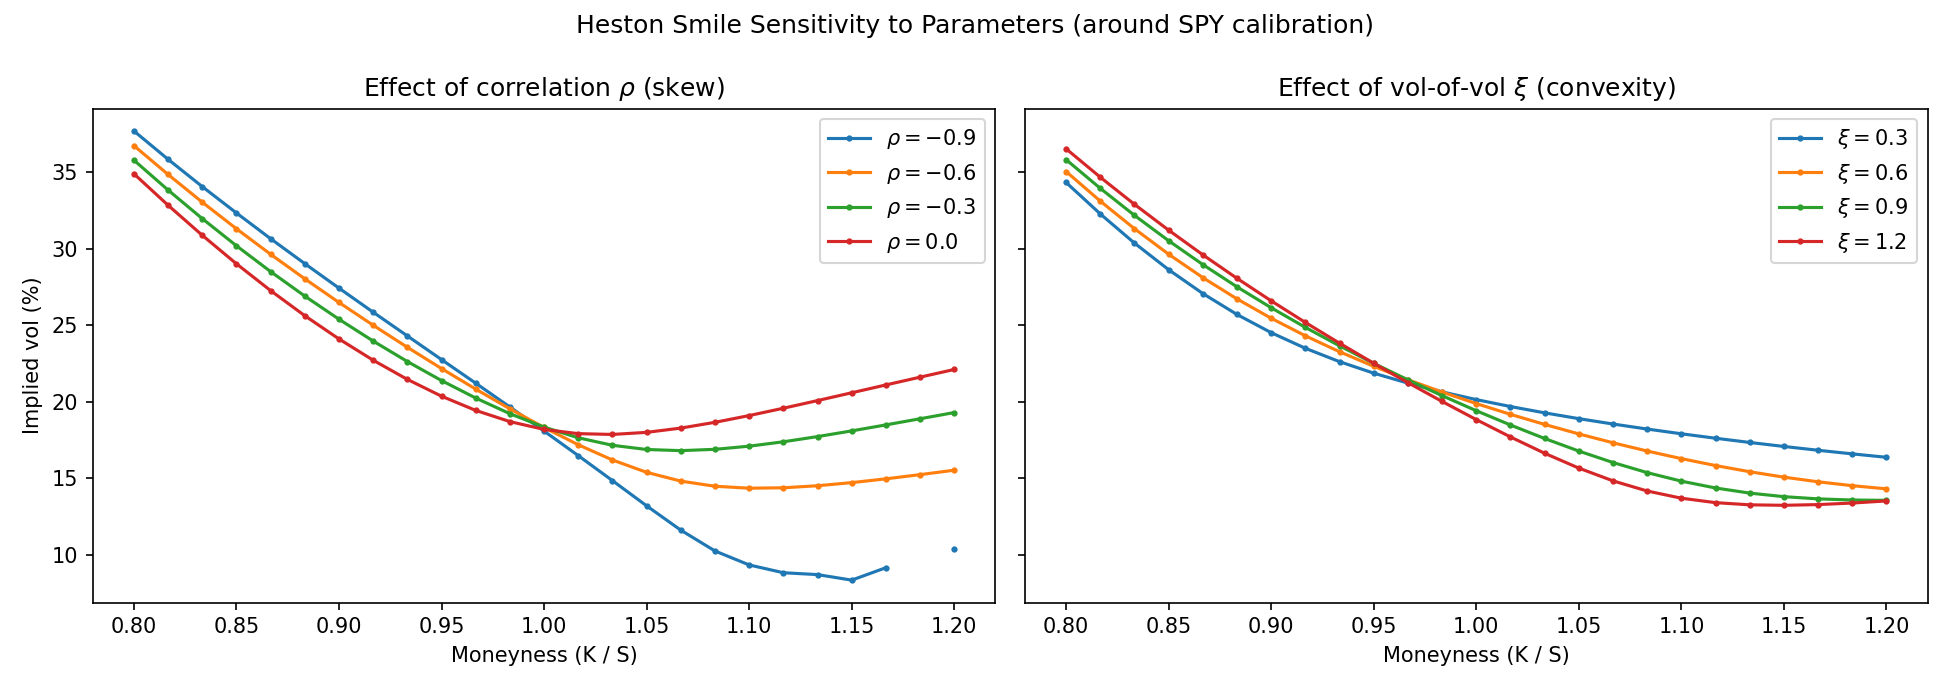
\includegraphics[width=\textwidth]{smile_sensitivity.png}
\caption{Heston smile sensitivity. Left: the correlation $\rho$ controls the
sign and steepness of the skew. Right: the vol-of-vol $\xi$ controls the
convexity of the smile.}
\label{fig:sensitivity}
\end{figure}

\section{Path-Dependent and American Options}
\label{sec:exotic}

\subsection{Exotics by Monte Carlo}
Options whose payoff depends on the whole price path generally lack closed forms,
making simulation the natural tool.

\paragraph{Asian options.} For an arithmetic-average Asian option no closed form
exists, but the \emph{geometric}-average version does---the geometric mean of
log-normals is log-normal---giving a Black--Scholes-type formula. We use it as a
control variate: the arithmetic and geometric payoffs are over $0.99$ correlated,
so subtracting the geometric control (with its analytic mean) cuts the standard
error by roughly $36\times$ at fixed sample size (Section~\ref{sec:results}).

\paragraph{Barrier options.} Knock-in and knock-out options are priced by
monitoring simulated paths against the barrier. We validate the estimator through
\emph{in--out parity}: a knock-in plus the corresponding knock-out must equal the
vanilla option, since on every path exactly one of the two pays. The simulated
sum matches the analytic vanilla price to within Monte Carlo error.

\paragraph{Lookback options.} Floating-strike lookbacks pay relative to the
path's running extremum and, as expected, are worth strictly more than the
corresponding vanilla option---a monotonicity the test suite enforces.

\subsection{American options by Least-Squares Monte Carlo}
American options permit early exercise, requiring the holder to compare immediate
intrinsic value against the (unknown) continuation value at each date. The
Longstaff--Schwartz algorithm \citep{longstaff2001} estimates the continuation
value by least-squares regression of discounted future cash flows on a polynomial
basis of the current spot, restricted to in-the-money paths, then applies the
resulting exercise policy by backward induction. For an American put our LSM
estimate agrees with a high-resolution binomial lattice to within simulation
error (Section~\ref{sec:results}), confirming both implementations.

The early-exercise decision is summarised by the \emph{exercise boundary}
$S^*(t)$: the critical spot below which (for a put) immediate exercise dominates
holding. Figure~\ref{fig:boundary} extracts this boundary from the lattice. It
lies strictly below the strike, rises monotonically toward $K$ as maturity
approaches---reflecting the shrinking time value that early exercise forgoes---and
meets the strike at expiry. The region beneath the curve is where the American
option is worth more dead than alive, the precise locus that distinguishes it
from its European counterpart.

\begin{figure}[H]
\centering
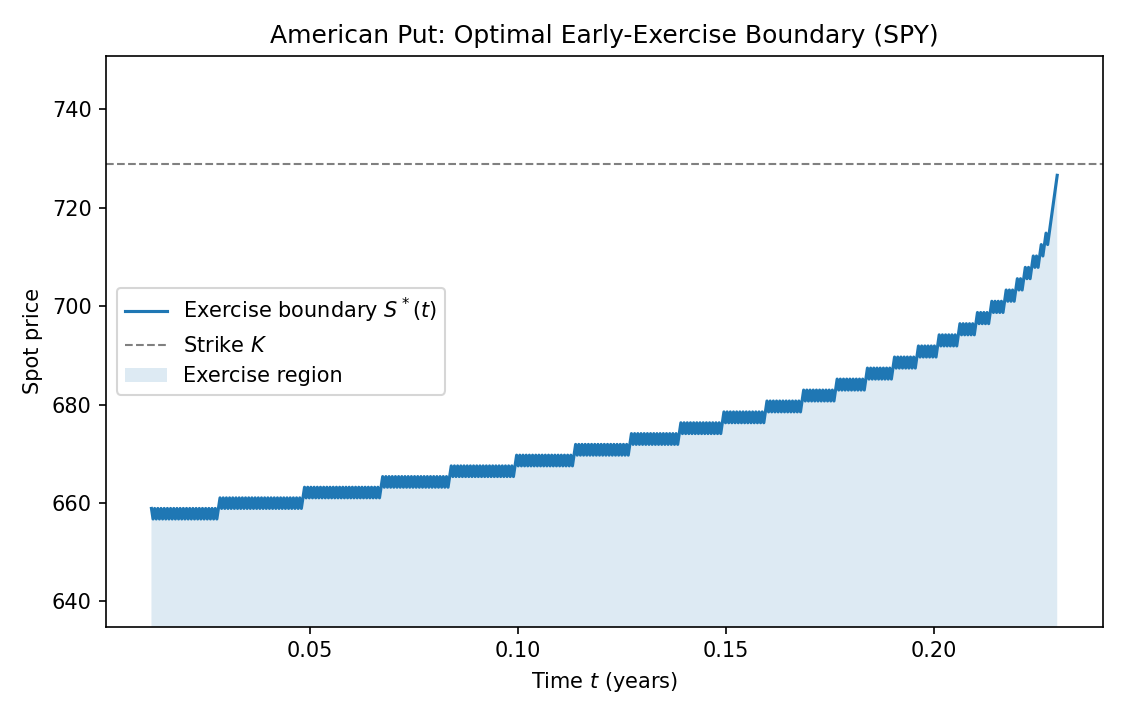
\includegraphics[width=0.72\textwidth]{exercise_boundary.png}
\caption{Optimal early-exercise boundary $S^*(t)$ for an American put on the SPY
reference contract ($K=729$, $T=0.23$, $\sigma=16.7\%$), extracted from the
binomial lattice. Exercise is optimal in the shaded region below the boundary;
the boundary rises to the strike at expiry. The staircase pattern reflects the
discrete lattice nodes.}
\label{fig:boundary}
\end{figure}

\section{Empirical Application: Calibration to S\&P~500 Options}
\label{sec:empirical}

\subsection{Data}
We take the full option chain on the SPDR S\&P~500 ETF (SPY) from Yahoo Finance,
recorded with the spot at \$728.99 (close of 2026-06-26). The risk-free rate
$r=3.66\%$ is the 13-week US Treasury-bill yield; for each expiry the forward $F$
is implied directly from put-call parity, which fixes the carry
$q=r-\ln(F/S)/T$ without a separate dividend assumption and makes the put and
call wings consistent at the money. We retain liquid out-of-the-money quotes only
(positive bid/ask, relative spread below $20\%$, open interest $\geq 25$,
moneyness in $[0.85,1.15]$): puts below the forward and calls above it. This
yields \textbf{903 quotes across six maturities} from 21 to 126 days. The
resulting implied-volatility skew (Figure~\ref{fig:marketsmile}) is the classic
equity-index shape: out-of-the-money puts trade $10$--$20$ volatility points
above out-of-the-money calls, and the skew is steepest at the shortest maturity
and flattens with $T$.

\begin{figure}[H]
\centering
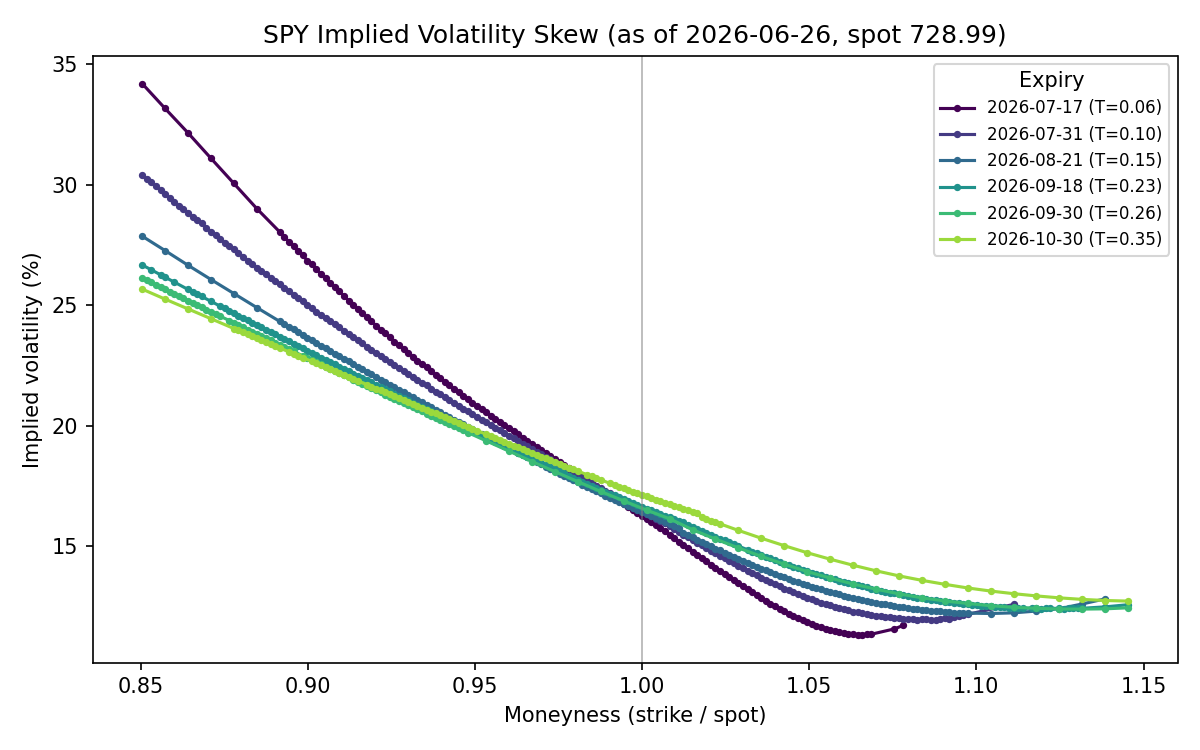
\includegraphics[width=0.78\textwidth]{market_smile.png}
\caption{Market implied-volatility skew of SPY options (as of 2026-06-26, spot
\$728.99), one curve per expiry. The pronounced negative skew and its
flattening with maturity are exactly the features Black--Scholes cannot
represent.}
\label{fig:marketsmile}
\end{figure}

\subsection{Calibration}
Calibration is the inverse problem of pricing: given the market quotes, find the
model parameters that reproduce them. We minimise the vega-weighted squared
pricing error
\begin{equation}
\min_{\Theta} \sum_{i} w_i^2
\left(C^{\text{model}}(K_i,T_i;\,\Theta)-C^{\text{mkt}}_i\right)^2,
\qquad w_i = 1/\mathcal{V}_i,
\end{equation}
by the Trust-Region Reflective least-squares method with parameter bounds. The
vega weighting $w_i=1/\mathcal{V}_i$ converts each dollar residual into an
approximate implied-volatility residual, so the cheap out-of-the-money options
that define the skew are not swamped by expensive at-the-money ones. We calibrate
the five Heston parameters $(v_0,\kappa,\theta,\xi,\rho)$ and the four Merton
parameters $(\sigma,\lambda,\mu_J,\sigma_J)$ to the same 903 quotes; the
resulting fits are shown in Figure~\ref{fig:calib} and Table~\ref{tab:calib}.

\begin{table}[H]
\centering
\caption{Calibrated parameters and fit quality on the 903 SPY quotes. ``Vol
RMSE'' is the root-mean-square error in Black--Scholes implied-volatility points.}
\label{tab:calib}
\begin{tabular}{lll}
\toprule
\multicolumn{2}{l}{\textbf{Heston}} & \textbf{Vol RMSE $=0.60\%$} \\
\midrule
$v_0=0.0259$ & $\kappa=8.89$ & $\theta=0.0416$ \\
$\xi=1.48$ & $\rho=-0.71$ & (Feller $2\kappa\theta>\xi^2$ violated) \\
\midrule
\multicolumn{2}{l}{\textbf{Merton}} & \textbf{Vol RMSE $=1.22\%$} \\
\midrule
$\sigma=0.111$ & $\lambda=0.85\,\text{yr}^{-1}$ & \\
$\mu_J=-0.130$ & $\sigma_J=0.085$ & \\
\bottomrule
\end{tabular}
\end{table}

The economic content of the estimates is exactly what the skew implies. Heston's
correlation $\rho=-0.71$ is strongly negative---the leverage effect that tilts
the smile downward---and Merton's mean jump $\mu_J=-0.13$ with intensity
$\lambda=0.85\,\text{yr}^{-1}$ encodes the market's pricing of sudden downward
moves (crash risk). Heston fits the surface markedly better than Merton ($0.60\%$
vs.\ $1.22\%$ vol RMSE): as Figure~\ref{fig:calib} shows, its two
skew-shaping parameters track the smile across maturities, whereas Merton's
fit deteriorates in the wings and at the shortest maturity, where even Heston
cannot fully match the steepness---a documented limitation of diffusive
stochastic-volatility models at short horizons. The calibrated $\kappa$ is the
least well-identified parameter, a known near-degeneracy with $\xi$ and $\theta$.

\begin{figure}[H]
\centering
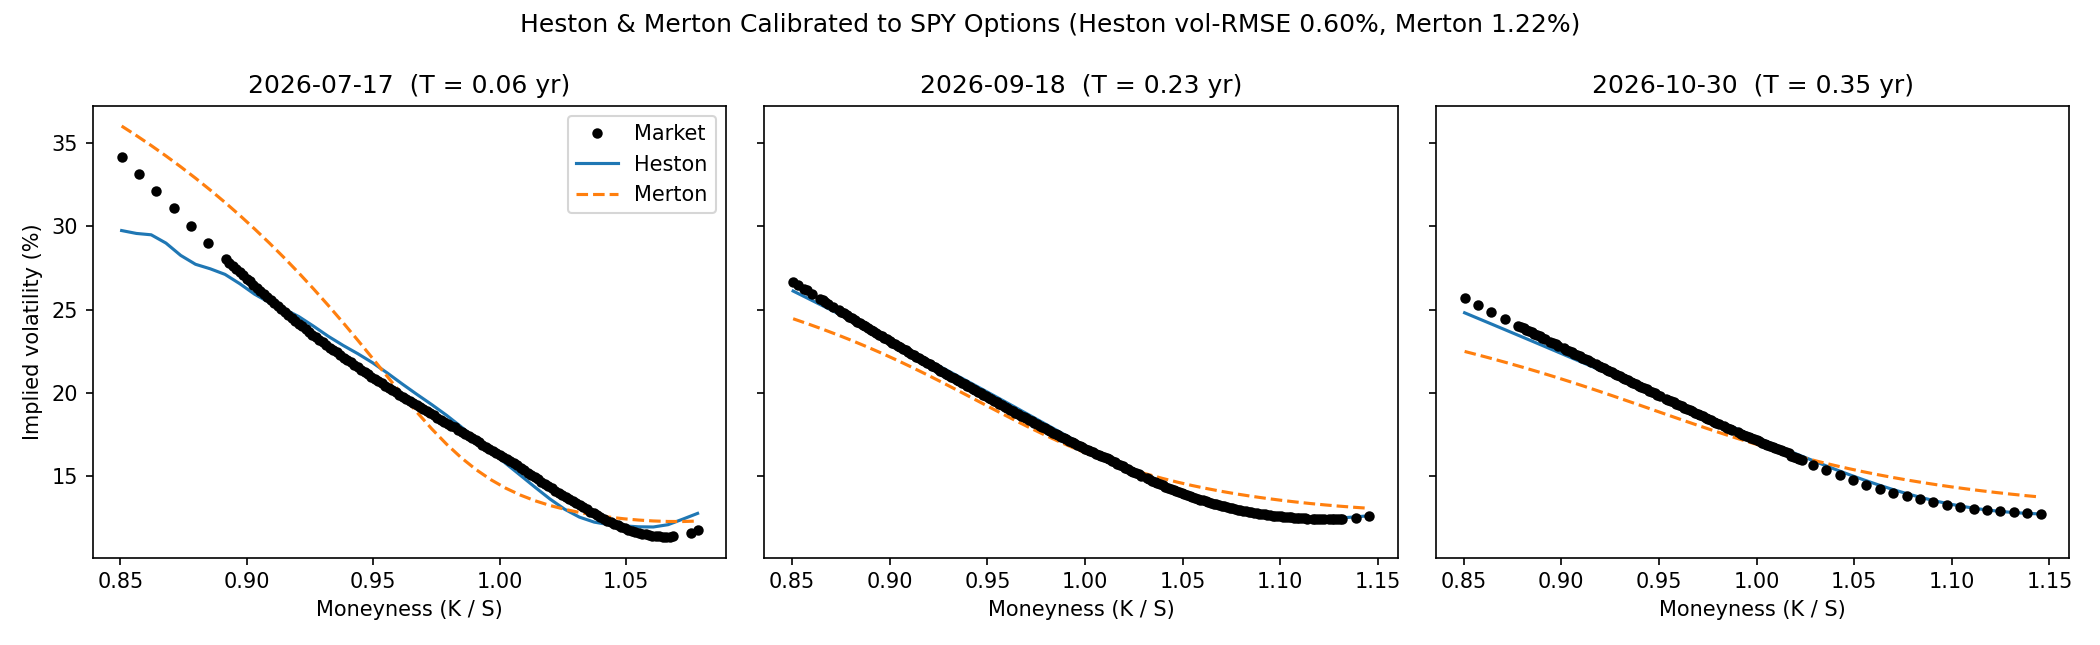
\includegraphics[width=\textwidth]{calibration_fit_real.png}
\caption{Heston and Merton calibrated to SPY options at three maturities. Markers
are market implied volatilities; lines are the calibrated models. Heston (solid)
fits the skew tightly except at the extreme short-dated wings; Merton (dashed)
captures the level but underfits the curvature.}
\label{fig:calib}
\end{figure}

\section{Numerical Results}
\label{sec:results}

All experiments use the real SPY reference contract: a near-at-the-money option
with $S_0=728.99$, $K=729$, $T=0.23$, $r=3.66\%$, the parity-implied carry
$q=-2.12\%$, and at-the-money implied volatility $\sigma=16.65\%$.
Table~\ref{tab:benchmark} collects the European call across the four numerical
methods; all agree to within Monte Carlo error, validating the implementations
against one another. Table~\ref{tab:advanced} reports the advanced-model
cross-checks, each priced two independent ways on the same contract.

\begin{table}[H]
\centering
\caption{European call on the real SPY contract ($S_0=728.99$, $K=729$,
$T=0.23$, $r=3.66\%$, $q=-2.12\%$, $\sigma=16.65\%$). ``SE'' is the Monte Carlo
standard error.}
\label{tab:benchmark}
\begin{tabular}{lcc}
\toprule
Method & Price & Note \\
\midrule
Black--Scholes (closed form) & 28.334 & benchmark \\
Binomial tree (500 steps)    & 28.322 & $O(1/N)$ convergence \\
Monte Carlo (200k paths)     & 28.338 & SE $=0.038$ \\
Quasi-Monte Carlo (Sobol, $2^{16}$) & 28.333 & error $7\times10^{-4}$ \\
\bottomrule
\end{tabular}
\end{table}

\begin{table}[H]
\centering
\caption{Cross-validation of the advanced models on the SPY contract using the
calibrated parameters. Each row prices the same contract two independent ways;
``SE'' is the Monte Carlo standard error. Prices differ across rows because each
model is priced with its own calibrated (full-smile) parameters, not the single
at-the-money volatility.}
\label{tab:advanced}
\begin{tabular}{lllcc}
\toprule
Model & Method A & Method B & A & B \\
\midrule
Heston call & Fourier & Monte Carlo & 28.545 & $28.732\pm0.067$ \\
Merton call & Series & Monte Carlo & 27.990 & $27.996\pm0.045$ \\
American put & Lattice & LSM & 19.500 & $19.505\pm0.077$ \\
\bottomrule
\end{tabular}
\end{table}

The variance-reduction and convergence experiments are summarised in the figures,
all computed on the real SPY contract.
Figure~\ref{fig:binomial} shows the binomial tree converging to Black--Scholes.
Figure~\ref{fig:mcvar} shows antithetic-plus-control-variate Monte Carlo
dominating plain Monte Carlo at every sample size. Figure~\ref{fig:qmc} shows the
quasi-Monte Carlo convergence-rate improvement. The market smile, calibrated
surface, and calibration-fit figures appear in
Sections~\ref{sec:beyond} and~\ref{sec:empirical}.

\begin{figure}[H]
\centering
\begin{subfigure}{0.49\textwidth}
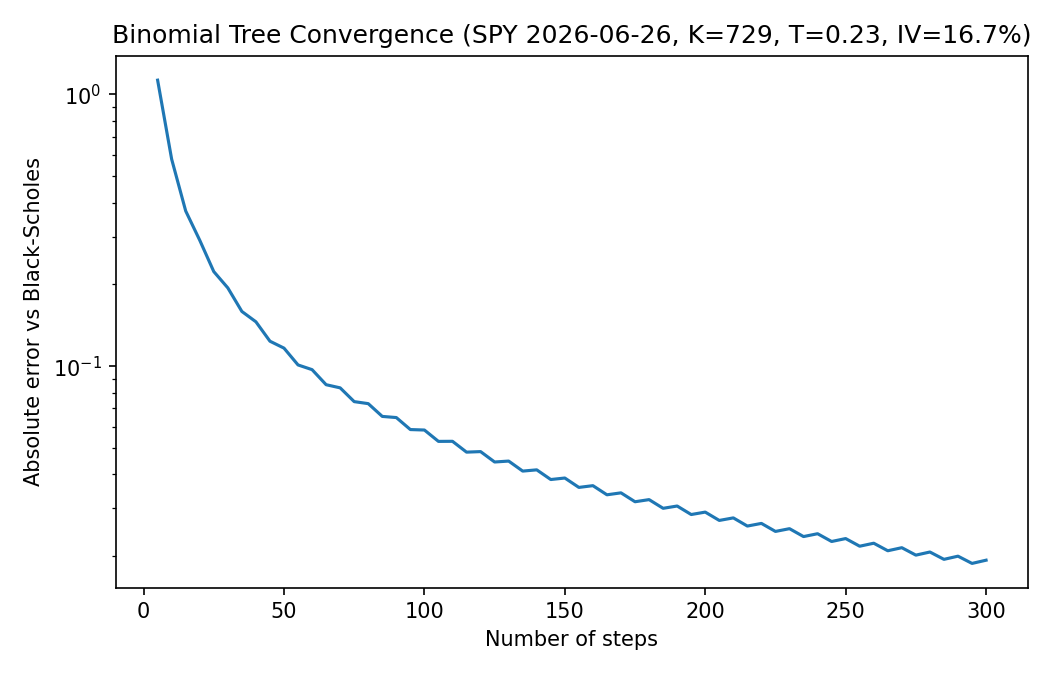
\includegraphics[width=\textwidth]{binomial_convergence.png}
\caption{Binomial tree convergence to BSM.}
\label{fig:binomial}
\end{subfigure}\hfill
\begin{subfigure}{0.49\textwidth}
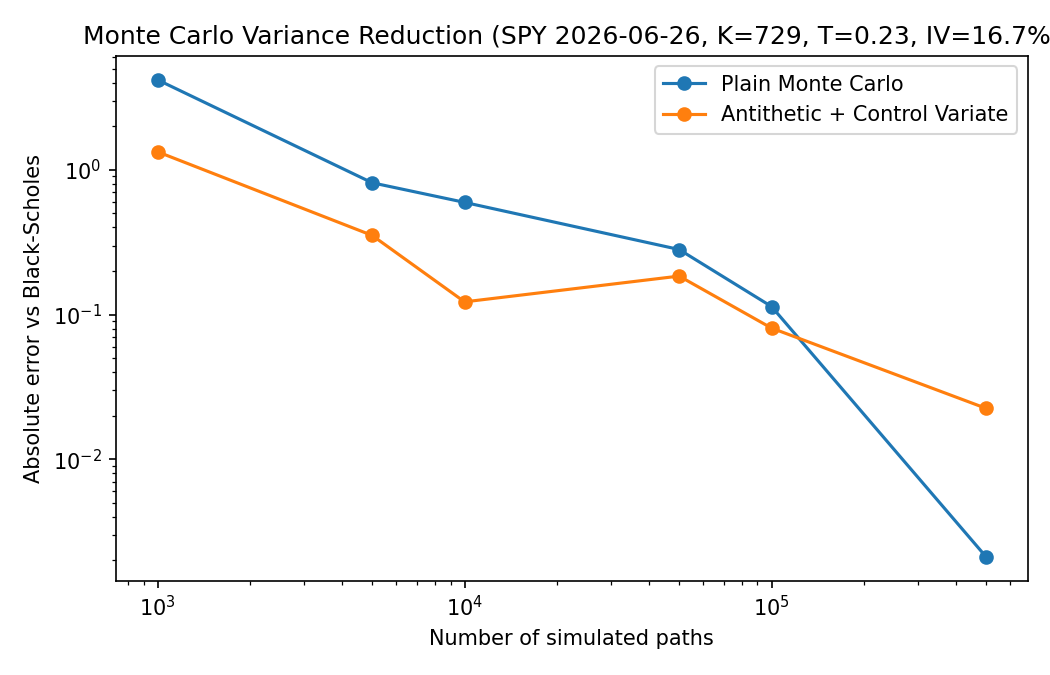
\includegraphics[width=\textwidth]{mc_variance_reduction.png}
\caption{Monte Carlo variance reduction.}
\label{fig:mcvar}
\end{subfigure}
\caption{Convergence and variance reduction for the European benchmark.}
\end{figure}

\begin{figure}[H]
\centering
\begin{subfigure}{0.49\textwidth}
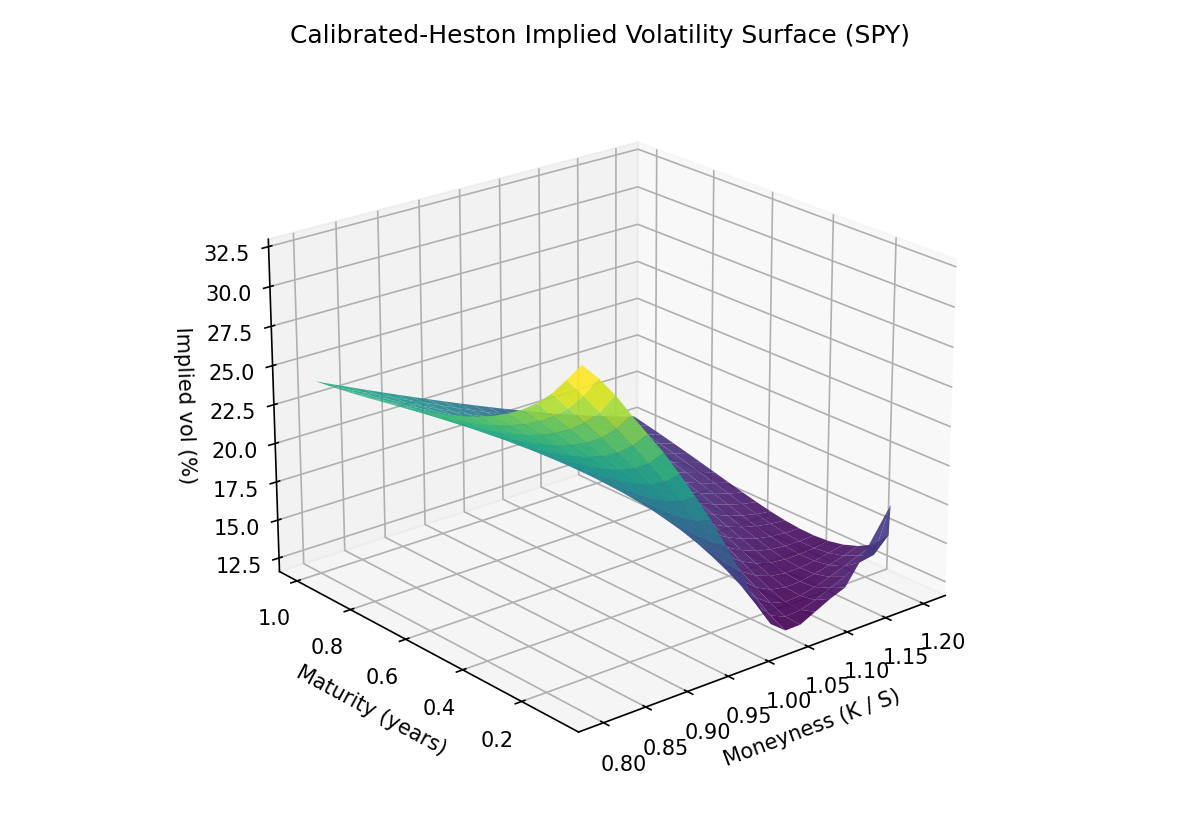
\includegraphics[width=\textwidth]{heston_surface.png}
\caption{Calibrated-Heston implied-volatility surface.}
\label{fig:surface}
\end{subfigure}\hfill
\begin{subfigure}{0.49\textwidth}
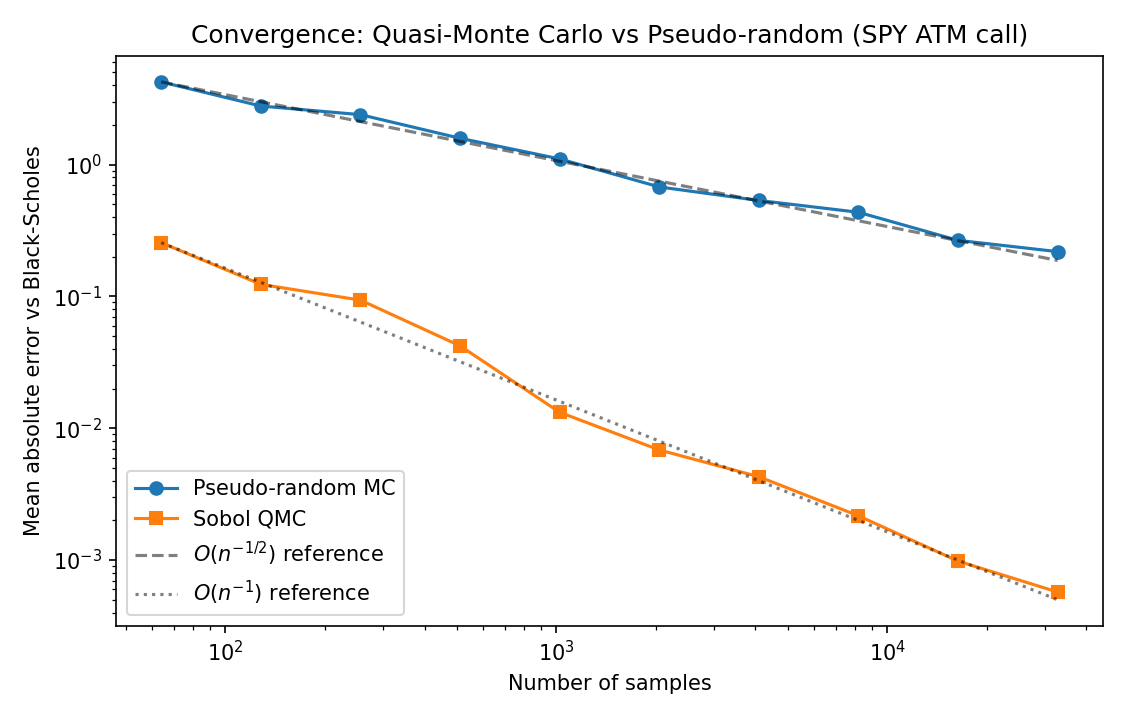
\includegraphics[width=\textwidth]{qmc_convergence.png}
\caption{QMC vs.\ pseudo-random convergence.}
\label{fig:qmc}
\end{subfigure}
\caption{Left: the SPY-calibrated Heston surface---skew steepest at short
maturities, flattening with $T$. Right: Sobol QMC error tracks $O(n^{-1})$ while
pseudo-random MC tracks $O(n^{-1/2})$.}
\end{figure}

\section{Conclusion}
\label{sec:conclusion}

We have built and empirically validated a hierarchy of option-pricing models and
numerical methods, organised around the failure of the Black--Scholes
constant-volatility assumption, and applied to real S\&P~500 option data. The
Heston and Merton models reproduce the market volatility skew and its term
structure that Black--Scholes cannot; semi-analytic Fourier pricing,
variance-reduced and quasi-Monte Carlo simulation, and regression-based American
exercise make these models computationally tractable; and calibration to live
quotes closes the loop from market data back to model parameters. The recurring
theme is cross-validation: each price is confirmed by an independent method, which
is both a correctness discipline and, for a practitioner, a source of confidence
in the numbers.

The principal quantitative findings, all on real SPY data, are:
\begin{itemize}
\item Calibrated to 903 liquid SPY quotes across six maturities, Heston fits the
market skew to $0.60\%$ implied-volatility RMSE and Merton to $1.22\%$
(Table~\ref{tab:calib}, Figure~\ref{fig:calib}); the estimated $\rho=-0.71$ and
mean jump $\mu_J=-0.13$ quantify the market's leverage effect and crash-risk
pricing.
\item All four European methods agree on the real SPY call to within Monte Carlo
error (Table~\ref{tab:benchmark}); the Heston Fourier price, Merton series, and
American LSM price each match their independent counterpart to within one to three
standard errors (Table~\ref{tab:advanced}).
\item The correlation $\rho$ governs the skew and the vol-of-vol $\xi$ the
convexity of the Heston smile (Figure~\ref{fig:sensitivity}), and the calibrated
models' non-Gaussian return distributions (Figure~\ref{fig:returns}) are the
mechanism that generates the observed skew.
\item Variance reduction is highly effective: a geometric-Asian control variate
cuts the arithmetic-Asian standard error by roughly $36\times$, and Sobol QMC
improves the European convergence rate from $O(n^{-1/2})$ toward $O(n^{-1})$
(Figure~\ref{fig:qmc}).
\end{itemize}

Natural extensions include the Bates model (Heston with jumps), the SABR model
for interest-rate smiles, Andersen's Quadratic-Exponential scheme for unbiased
Heston simulation, stochastic local volatility for exact surface fitting, and
adjoint algorithmic differentiation for fast Greeks. All code, tests, and
figure-generating scripts are available in the companion repository.

\begin{thebibliography}{9}

\bibitem[Albrecher et al.(2007)]{albrecher2007}
Albrecher, H., Mayer, P., Schoutens, W., \& Tistaert, J. (2007).
The little Heston trap. \emph{Wilmott Magazine}, January, 83--92.

\bibitem[Black \& Scholes(1973)]{blackscholes1973}
Black, F., \& Scholes, M. (1973). The pricing of options and corporate
liabilities. \emph{Journal of Political Economy}, 81(3), 637--654.

\bibitem[Cox et al.(1979)]{crr1979}
Cox, J. C., Ross, S. A., \& Rubinstein, M. (1979). Option pricing: A simplified
approach. \emph{Journal of Financial Economics}, 7(3), 229--263.

\bibitem[Heston(1993)]{heston1993}
Heston, S. L. (1993). A closed-form solution for options with stochastic
volatility with applications to bond and currency options.
\emph{Review of Financial Studies}, 6(2), 327--343.

\bibitem[Longstaff \& Schwartz(2001)]{longstaff2001}
Longstaff, F. A., \& Schwartz, E. S. (2001). Valuing American options by
simulation: A simple least-squares approach.
\emph{Review of Financial Studies}, 14(1), 113--147.

\bibitem[Lord et al.(2010)]{lord2010}
Lord, R., Koekkoek, R., \& van Dijk, D. (2010). A comparison of biased simulation
schemes for stochastic volatility models. \emph{Quantitative Finance}, 10(2),
177--194.

\bibitem[Merton(1973)]{merton1973}
Merton, R. C. (1973). Theory of rational option pricing.
\emph{Bell Journal of Economics and Management Science}, 4(1), 141--183.

\bibitem[Merton(1976)]{merton1976}
Merton, R. C. (1976). Option pricing when underlying stock returns are
discontinuous. \emph{Journal of Financial Economics}, 3(1--2), 125--144.

\end{thebibliography}

\end{document}
